\documentclass{article}
\usepackage{amsmath}
\usepackage{amssymb}
\newcommand*{\qed}{\hfill\ensuremath{\blacksquare}}
\usepackage{graphicx}
\graphicspath{{.}}

\title{Computational Linear Algebra, Module 7}
\author{Maya Shende}
\date{Due: April 11th, 2018}

\begin{document}
\maketitle

\begin{enumerate}

%exercise 1
\item output:\\
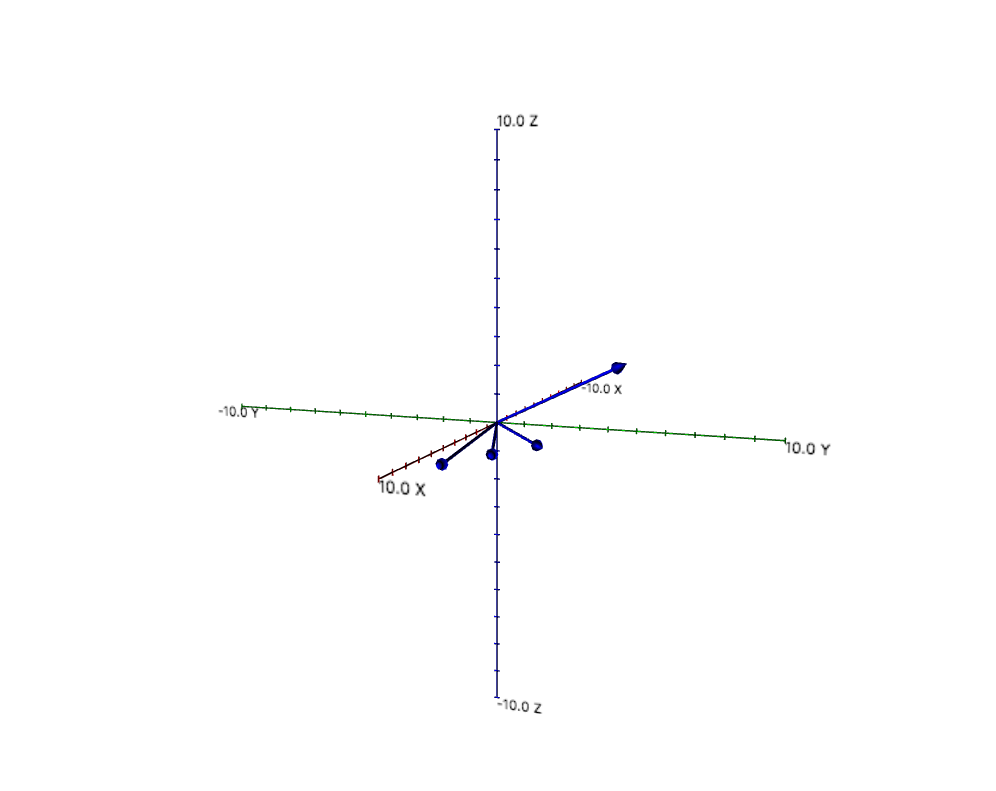
\includegraphics[scale=0.3]{exercise1}

%exercise 2
\item $c_3$ is not included in the linear combination because it is linearly dependent on the other two columns. \\
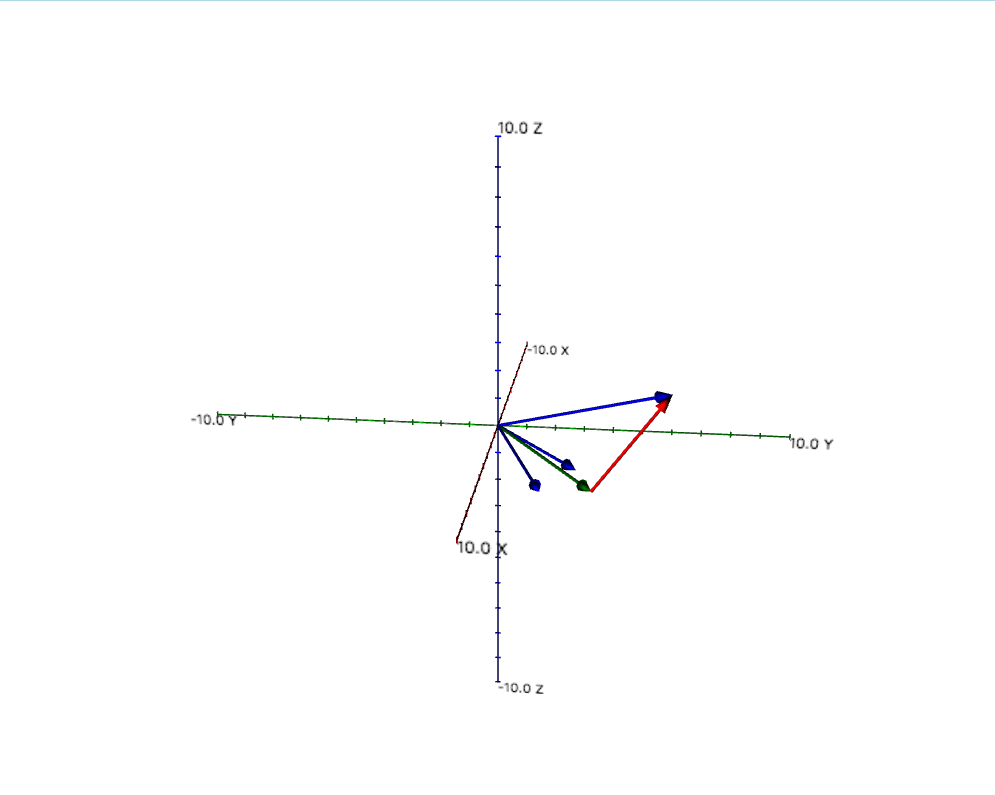
\includegraphics[scale=0.3]{exercise2_1}\\
If I increase the range, I get a $y$ vector that is a bit closer, in the sense that it is the same as $b$, but without the $z$ component. \\
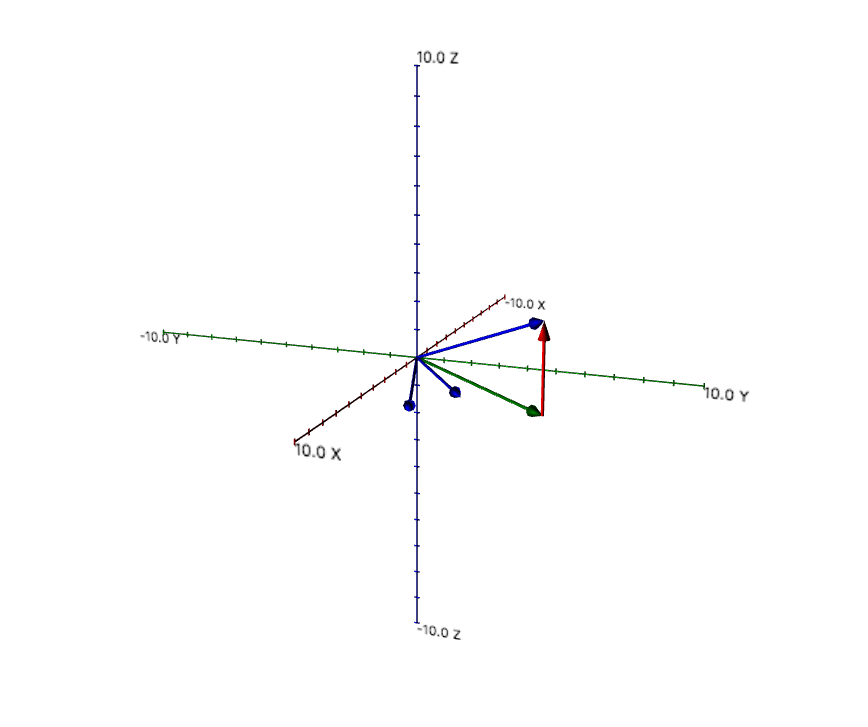
\includegraphics[scale=0.3]{exercise2_new_range}

need to insert drawing!

%exercise 3
\item We need to show that $AB < AC$ for all $AC$. We know that 
\begin{eqnarray*}
	AB^2 + BC^2 &=& AC^2\\
	AB^2 &=& AC^2 - BC^2\\
	AB^2 < AC^2\\
	AB &<& AC
\end{eqnarray*}
So, the shortest distance from the point to the plane is on the perpendicular to the plane. 

%exercise 4
\item Both $c_1$ and $c_2$ are in the $xy$-plane, with $z$ components of 0. So, the closest linear combination of them to $b$ will be the projection of $b$ on the $xy$-plane. Therefore, if we look at $\textbf{z}$, the vector form $y$ to $b$, since it is orthogonal to the projection, it is orthogonal to both $c_1$ and $c_2$. 

%exercise 5
\item Using the data in the example above and taking the dot product, the equations for $\alpha$ and $\beta$ are
\begin{eqnarray*}
	42 - 40\alpha - 30\beta &=& 0\\
	38 - 30\alpha -25\beta &=& 0
\end{eqnarray*}
and by solving these equations, we get $\alpha = \frac{-27}{30}$ and $\beta = \frac{13}{5}$. \\
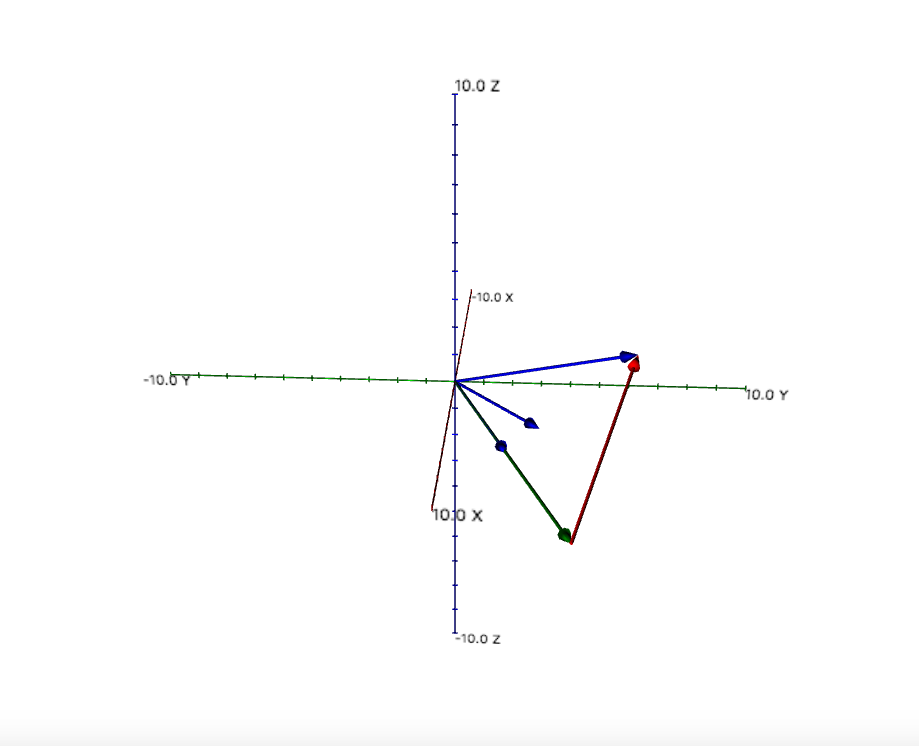
\includegraphics[scale=0.3]{exercise5}

%exercise 6
\item This works because of how matrix multiplication works. By have the $c$'s as rows, we are going to multiply each $c_i$ with $z_i$. 

%exercise 7
\item $B$ is the transpose of $A$. 

%exercise 8
\item 

%exercise 9
\item $A \rightarrow (m \times n)$, $A^T \rightarrow (n \times m)$, $A^TA \rightarrow (n \times n)$. So, \\
\begin{eqnarray*}
	(A^TA)^{-1}A^Tb &\rightarrow& (n \times n)(n \times m)(m \times 1)\\
	&\rightarrow& (n \times m)(m \times 1)\\
	&\rightarrow& (n \times 1)
\end{eqnarray*}

%exercise 10
\item 
\begin{eqnarray*}
	(A^TA)^{-1} &=& A^{-1}(A^T)^{-1}\\
	(A^TA)^{-1}A^T &=& A^{-1}(A^T)^{-1}A^T\\
	&=& A^{-1}\\
	(A^TA)^{-1}A^Tb &=& A^{-1}b
\end{eqnarray*}

%exercise 11
\item If $\textbf{A}^{-1}$ exists, the dimension and the column rank are equal. Since those two are equal, the row rank is also equal to the other two. This means that is $\textbf{A}^{-1}$ exists, then $\left(\textbf{A}^{T}\right)^{-1}$ must also exist.

%exercise 12
\item We have $AB^{-1} = B^{-1}A^{-1}$. Now, in exercise 10, if we replace $A^T$ with $A$ and $A$ with $B$, then we can use the same proof to prove Theorem 7.1. 

%exercise 13
\item Matrix (2x2):\\
	0.250 -0.300\\
	-0.300  0.400\\
	x[0]=-0.9000000000000004 x[1]=2.6000000000000014\\
	
	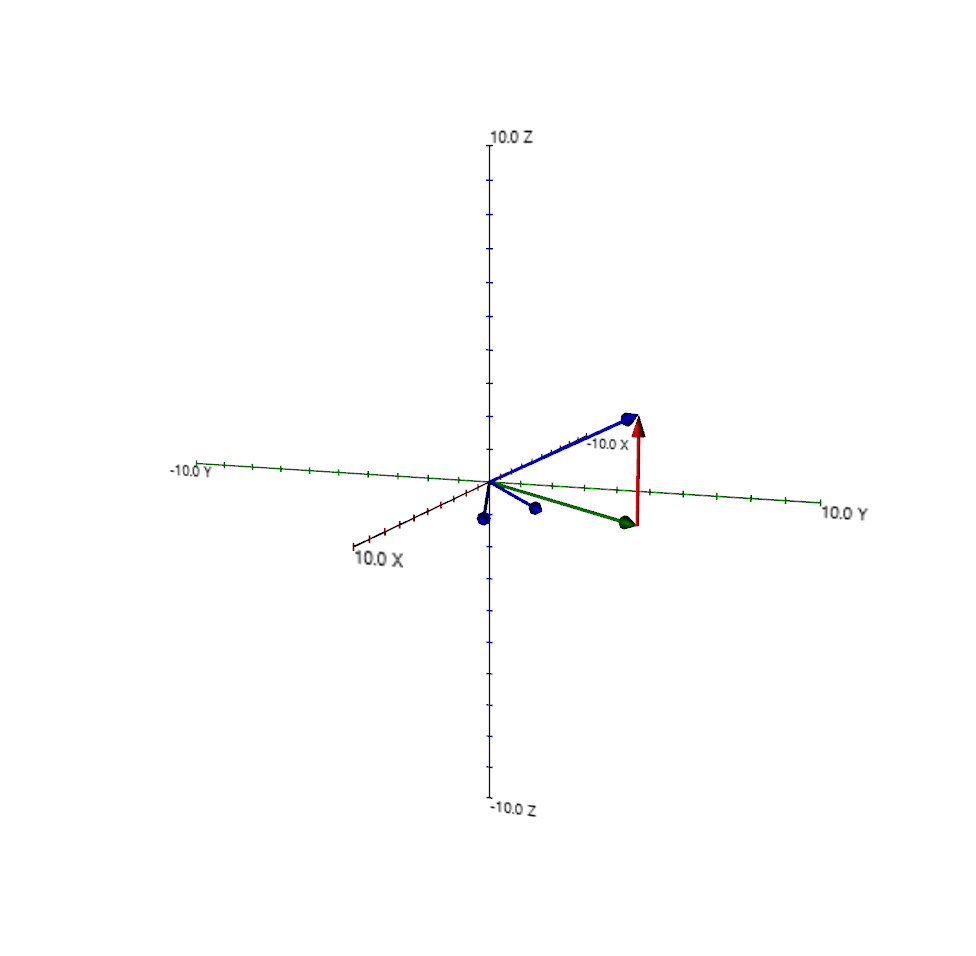
\includegraphics[scale=0.3]{module7_exercise13}

%exercise 14
\item The columns is not linearly independent because no inverse exists.


%exercise 15
\item Before:\\
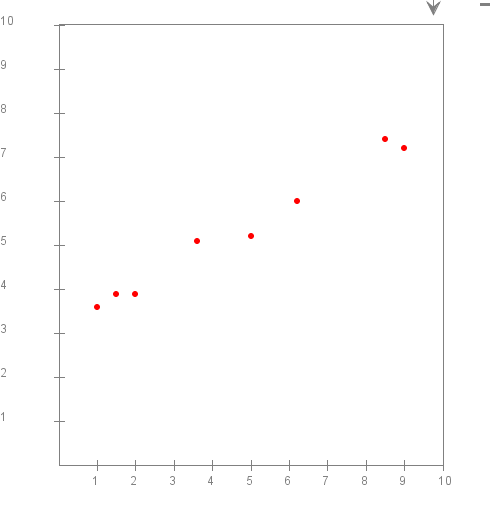
\includegraphics[scale=0.4]{module7_exercise15_a}\\
After:\\
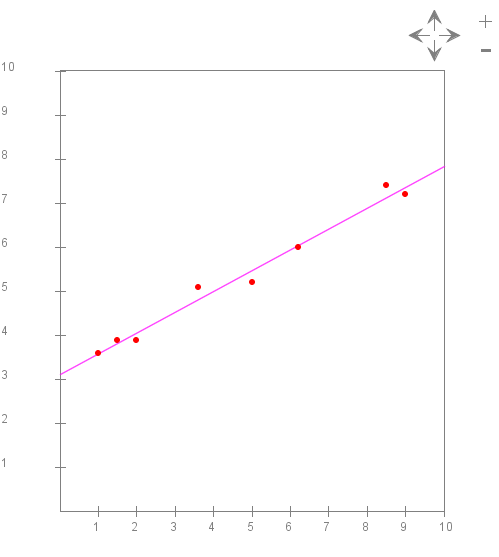
\includegraphics[scale=0.4]{module7_exercise15_b}

%exercise 16
\item Before:\\
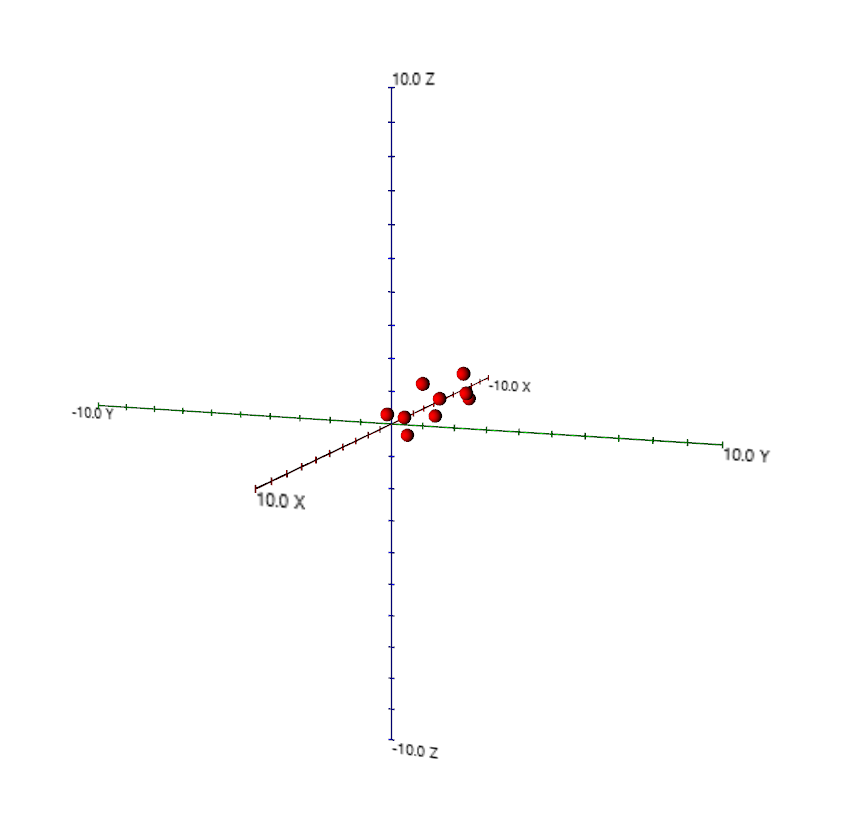
\includegraphics[scale=0.4]{module7_exercise16_a}\\
After:\\
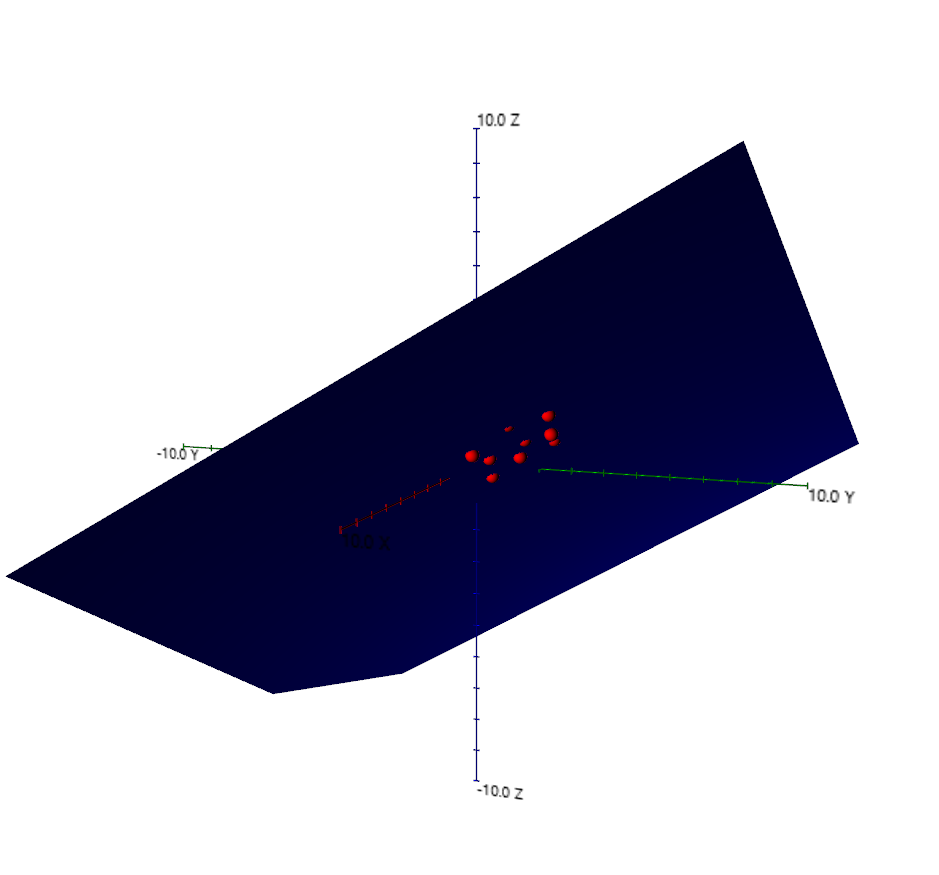
\includegraphics[scale=0.4]{module7_exercise16_b}

%exercise17
\item Before :\\
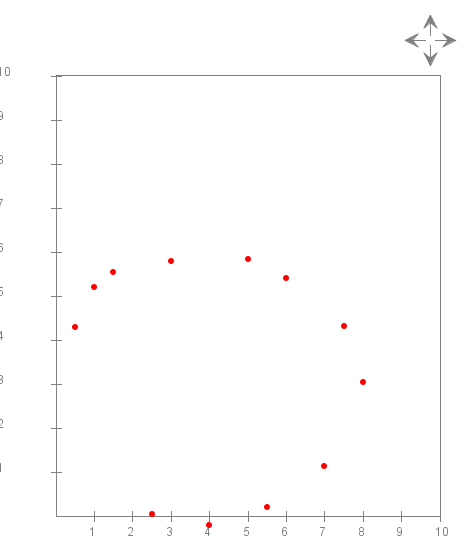
\includegraphics[scale=0.4]{module7_exercise17}\\
After:\\
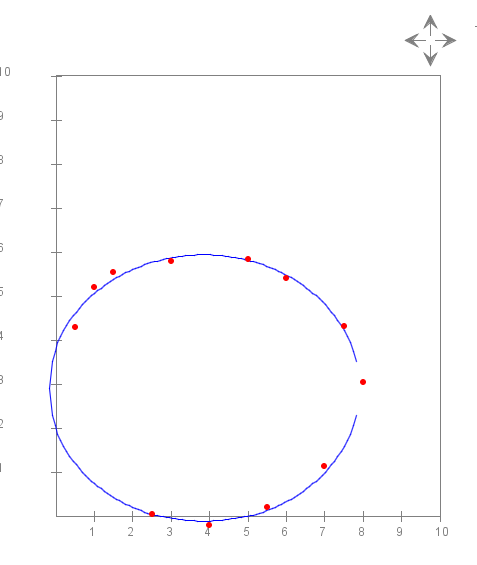
\includegraphics[scale=0.4]{module7_exercise17_b}

%exercise18
\item Before change of basis:\\
	meanX= 4.462, meanY= 4.575 varX= 5.846, varY= 6.505 covariance=49.260
	\\\\
	After change of basis:\\
	meanX= 4.519, meanY= 0.056 varX= 6.166, varY= 0.009 covariance= 1.319

%exercise 19
\item 
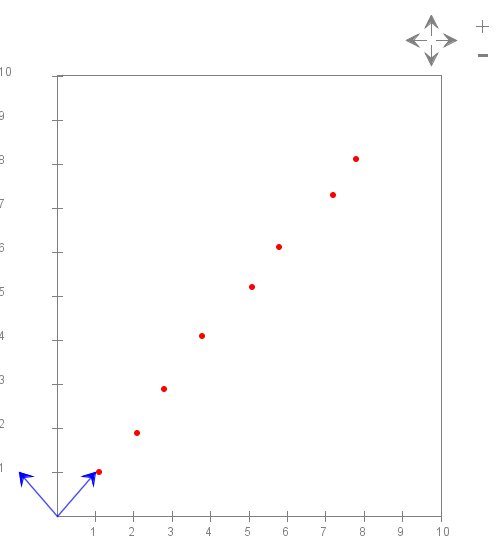
\includegraphics[scale=.5]{module7_exercise19}
	\\\\
	Coordinates after change of basis:\\
	( 1.050, -0.050)\\
	( 2.000, -0.100)\\
	( 2.850,  0.050)\\
	( 3.950,  0.150)\\
	( 5.150,  0.050)\\
	( 5.950,  0.150)\\
	( 7.250,  0.050)\\
	( 7.950,  0.150)

%exercise 20
\item $$ \alpha = \frac{\textbf{w} \cdot \textbf{v}}{\textbf{v} \cdot \textbf{v}} = \frac{(4)(6) + (3)(2)}{(6)(6) + (2)(2)} = \frac{30}{40} = \frac{3}{4}$$
	$$ \textbf{z} = \begin{bmatrix}4 \\ 3\end{bmatrix} - \frac{3}{4}\begin{bmatrix}6 \\ 2\end{bmatrix} = \begin{bmatrix}-0.5 \\ 1.5\end{bmatrix}$$
	$$ \textbf{z} \cdot \textbf{v} = (-0.5)(6) + (1.5)(2) = 0$$


%exercise 21
\item 
	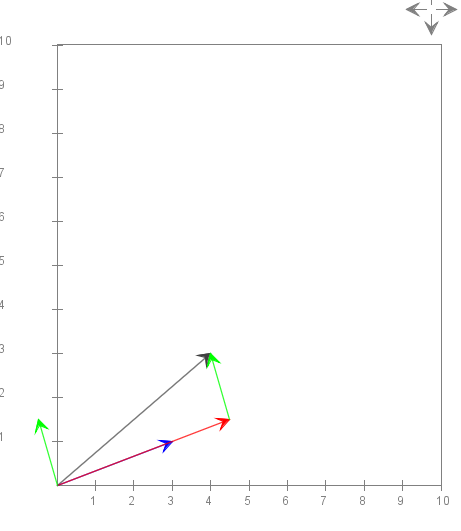
\includegraphics[scale=.5]{module7_exercise21}
	\\\\
	alpha = 1.5\\
	z=(-0.5,1.5)\\
	z dot v = 0.0\\
	\\\\
	The additional arrow is $\textbf{z}$.
	
%exercise 22
\item before:\\
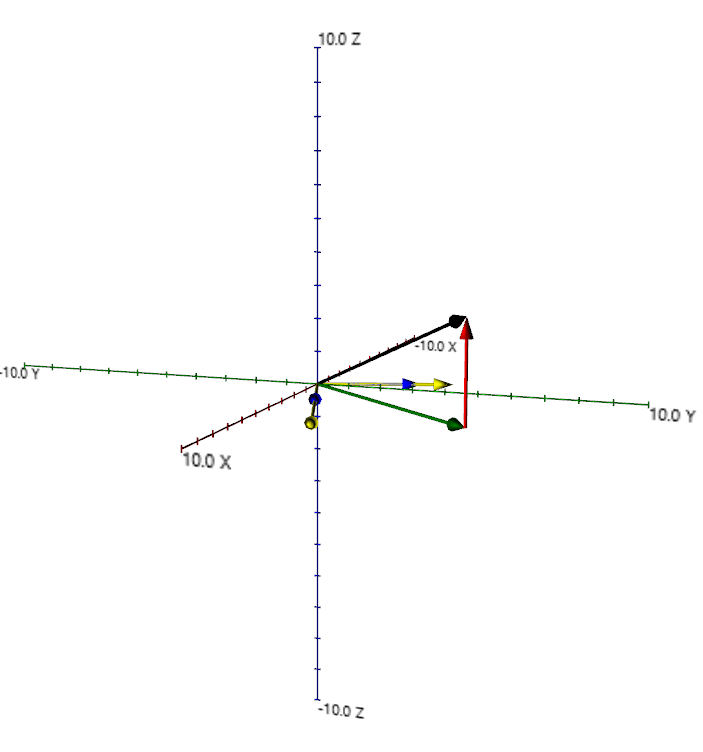
\includegraphics[scale=0.4]{module7_exercise22_a}\\
after:\\
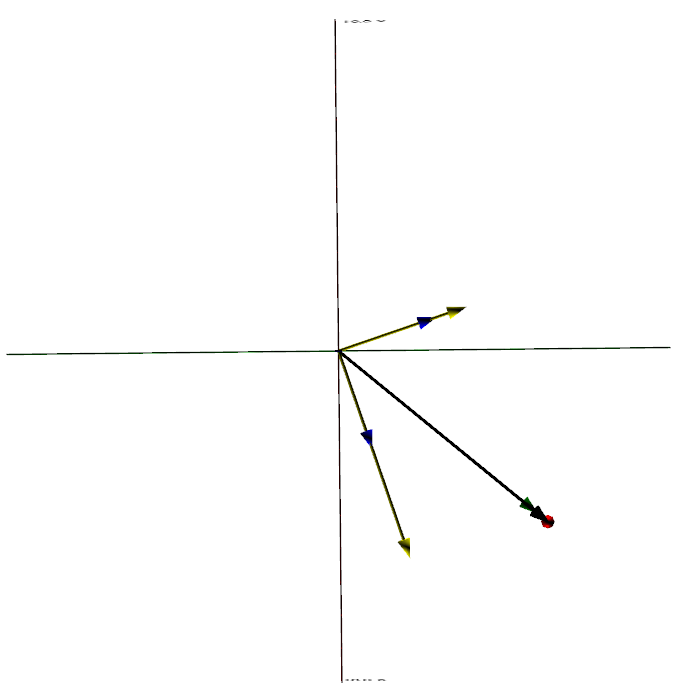
\includegraphics[scale=0.4]{module7_exercise22_b}
	z dot v1 = -2.6645352591003757E-15\\
	z dot v2 = 8.881784197001252E-16

%exercise23
\item
	\begin{itemize}
		\item $\textbf{v}_1 \cdot \textbf{v}_2 = (6)(-1) + (2)(3) = 0$	
		\item $\alpha_1 = \frac{(4)(6) + (2)(3)}{(6)(6) + (2)(2)} = .75$ and $\alpha_2 = \frac{(4)(-1) + (3)(3)}{(-1)(-1) + (3)(3)} = .5$
		\item $\text{proj}_{v_1} = .75 \begin{bmatrix}6\\2\end{bmatrix} = \begin{bmatrix}\frac{9}{2}\\\frac{3}{2}\end{bmatrix}$ and $\text{proj}_{v_2} = .5 \begin{bmatrix}-1\\3\end{bmatrix} = \begin{bmatrix}-\frac{1}{2}\\\frac{3}{2}\end{bmatrix}$
		\item $\textbf{w} = \begin{bmatrix}\frac{9}{2}\\\frac{3}{2}\end{bmatrix} + \begin{bmatrix}-\frac{1}{2}\\\frac{3}{2}\end{bmatrix} = \begin{bmatrix}4\\3\end{bmatrix}$
	\end{itemize}

%exercise 24
\item

%exercise 25
\item 

%exercise 26
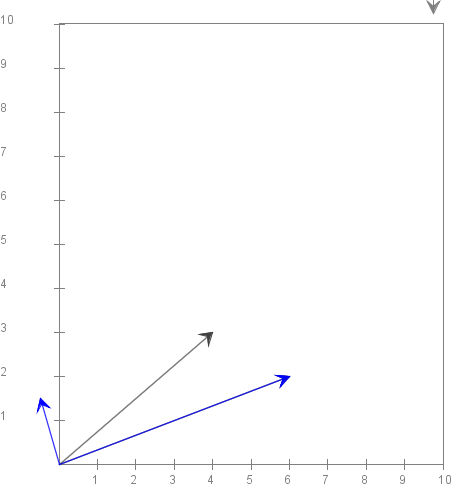
\includegraphics[scale=0.5]{module7_exercise26}

%exercise 27
\item 	
	v1 dot v2 = 3.552713678800501E-15\\
	v1 dot v3 = 5.329070518200751E-15\\
	v2 dot v3 = -3.552713678800501E-15
	
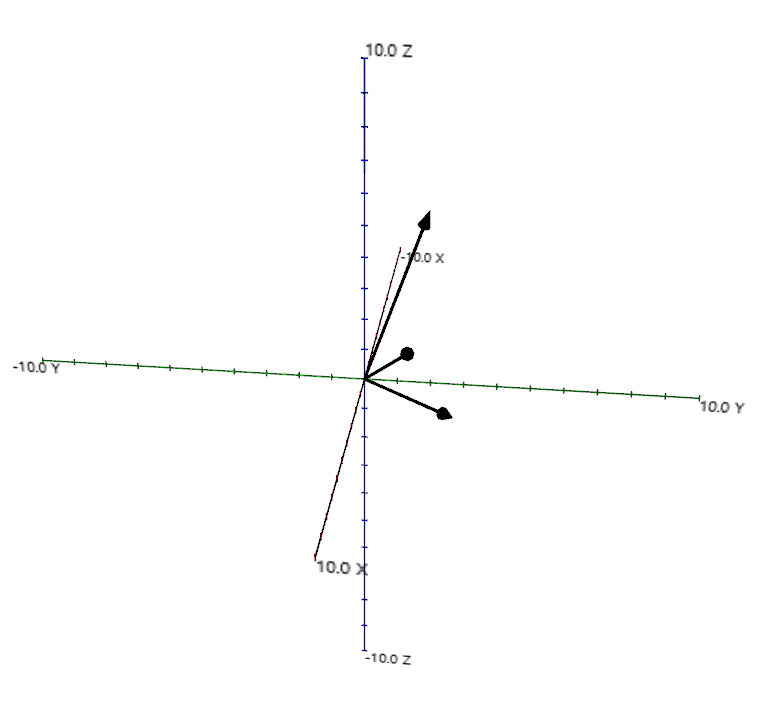
\includegraphics[scale=0.4]{module7_exercise27}\\
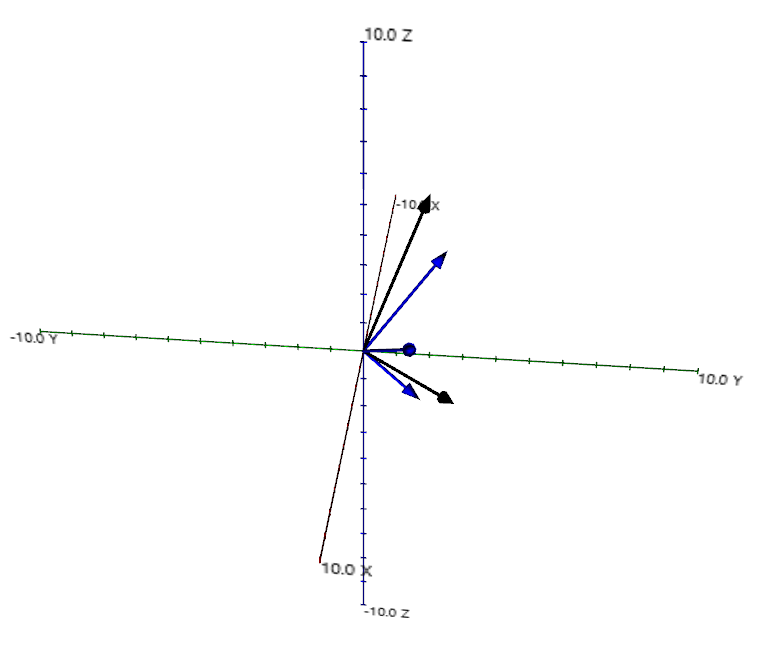
\includegraphics[scale=0.4]{module7_exercise27_b}



\end{enumerate}
\end{document}